\section{Auswertung}
\label{sec:Auswertung}

\subsection{Vorbereitung}\label{subsec:Vorbereitung}
Um die Messungen auswerten zu können, muss zunächst das Eigenträgheitsmoment $I_{D}$ und die Winkelrichtgröße $D$ berechnet werden.\\
\\
%Mit (\ref{eq:drehmoment}) und (\ref{eq:drehmomentwinkel}) ergibt sich:
%\begin{equation}
%D = \frac{\lvert F \rvert \lvert r \rvert \sin{\vartheta}}{\varphi} \stackrel{F,r > 0}{=} \frac{F r \sin{\vartheta}}{\varphi} 
%\stackrel{\vartheta = \frac{\pi}{2}}{=} \frac{F \cdot r}{\varphi}
%\end{equation}

In Tabelle (\ref{tab:Winkelrichtgröße}) sind die entsprechenden Messwerte und die berechneten Winkelrichtgrößen.

\begin{table}
\centering
\caption{Die Messdaten zu der Winkelrichtgröße bei $r = 20 \unit{\centi\meter}$.}
\label{tab:Winkelrichtgröße}
\begin{tabular}{c c c}
  \toprule
  $\varphi / °$  &  $F / \unit\newton$ & $D / \unit{\newton\meter}$ \\
  \midrule
              20 &        0,022 &     0,012605 \\
              30 &        0,054 &     0,020626 \\
              40 &        0,077 &     0,022059 \\
              50 &        0,092 &     0,021085 \\
              60 &        0,120 &     0,022918 \\
              70 &        0,144 &     0,023573 \\
              80 &        0,162 &     0,023205 \\
              90 &        0,188 &     0,023937 \\
             100 &        0,190 &     0,021772 \\
             110 &        0,200 &     0,020835 \\
             120 &        0,230 &     0,021963 \\
  \bottomrule
\end{tabular}
\end{table}

Es ergibt sich der Mittelwert:
\begin{align*}
  D_{mittel} = D  & = (0,021 \pm 0,003) \, \unit{\newton\meter} \text{ .}
\end{align*}

Um das Eigenträgheitsmoment zu bestimmen wird $I$ nach (\ref{eq:Tumgestellt1}) berechnet.
%Dafür wird die Umlaufzeit gemessen, wobei der Stab mit zwei bekannten Massen an den Seiten ausgelenkt wird.
%Dabei ist der Radius genau bestimmt.
Die Daten sind in Tabelle (\ref{tab:Eigenträgheitsmoment}) aufgetragen.

\begin{table}
  \centering
  \caption{Die Messdaten zum Eigenträgheitsmoment $I_{D}$}
  \label{tab:Eigenträgheitsmoment}
  \begin{tabular}{c c c c}
    \toprule
    $r / \unit\meter$  &  $T / \unit\second$ & $r^2 / (\unit\meter^2)$  & $T^2 / (\unit\second)^2$\\
    \midrule
      0,050   & 2,750   & 0,003   &  7,562  \\
      0,075   & 3,100   & 0,006   &  9,610  \\
      0,100   & 3,800   & 0,010   & 14,440  \\
      0,125   & 4,100   & 0,016   & 16,810  \\
      0,150   & 4,750   & 0,022   & 22,562  \\
      0,175   & 5,300   & 0,031   & 28,090  \\
      0,200   & 5,800   & 0,040   & 33,640  \\
      0,225   & 6,600   & 0,051   & 43,560  \\
      0,250   & 7,150   & 0,062   & 51,123  \\
      0,275   & 7,800   & 0,076   & 60,840  \\
    \bottomrule
    \end{tabular}
\end{table}

Aus diesen Daten wird das Eigenträgheitsmoment bestimmt.
Aufgrund der Form der verwendeteten Gewichte wird zunächst noch die Formel für einen Zylinder benötigt,
welche sich rechnerisch bestimmen lässt zu
\begin{equation*}
  I_{\text{Zyl}} = \frac{m \cdot R^2} {2} \text{ .}
\end{equation*}

Mit dem Satz von Steiner aus (\ref{eq:SatzvSteiner}) ergibt sich
\begin{equation} \label{eq:IZyl}
  I_{\text{Zyl}} = I_{D} + m_{\text{Zyl}}  \left( \frac{3 r^2 + h^2}{6} \right) \text{ .}
\end{equation}

Nach Einsetzen von $I_{\text{Zyl}}$ in Gleichung (\ref{eq:Tumgestellt1}) und Umstellen, ergibt sich:

\begin{equation}
  T^2 = \frac{4 \pi^2}{D} \cdot \left( 2ma^2 + I_{\text{Zyl}} \right) \stackrel{(\ref{eq:IZyl})}{=} 
  \frac{4 \pi^2}{D} \left( ma^2 + I_{D} + m_{\text{Zyl}}  \left( \frac{3 r^2 + h^2}{6} \right) \right)
\end{equation}

Durch lineare Regression mithilfe der Ausgleichsgerade 
\begin{equation*}
  y = a \cdot x + b 
\end{equation*}

mit den Parametern $a = 724,885 ± 10,115 \frac{1}{\unit{\square\second\square\meter}}$ und $b = 5,945 ± 0,400\frac{1}{\unit{\square\second}}$ ergibt sich der Plot in Abbildung (\ref{fig:Lineareregression}).

\begin{figure}[H]
  \centering
  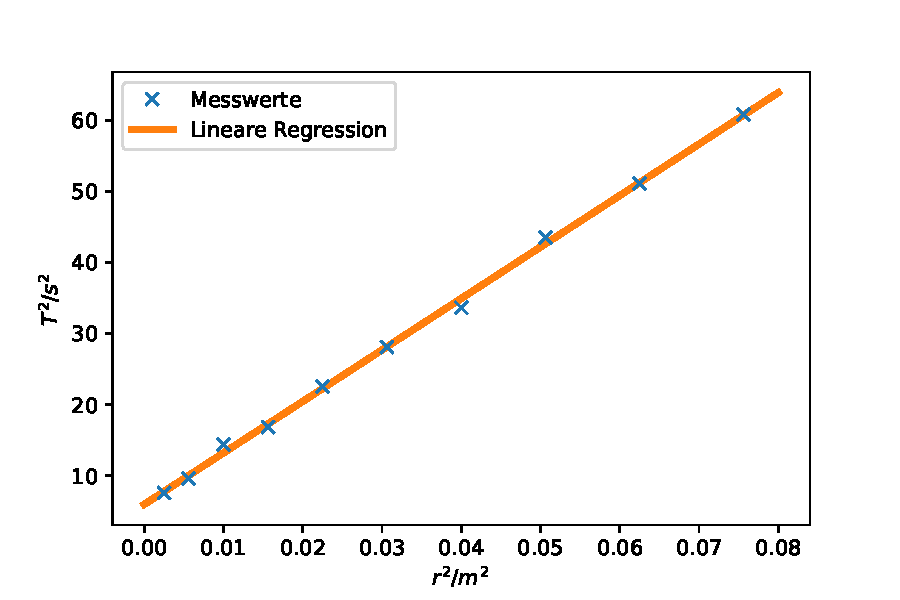
\includegraphics{pictures/Lineare Regression.pdf}
  \caption{Regressionsgerade des Eigenträgheitsmomentes}
  \label{fig:Lineareregression}
\end{figure}

Nun wird durch Koeffizientenvergleich a und b in (\ref{eq:IZyl}) erkannt und eingesetzt.
Es ergibt sich:
\begin{align} \label{var:aundb}
  a & = \frac{8 \pi^2 m}{D} & b & = \frac{4 \pi^2}{D} \left(I_{D} + m_{\text{Zyl}} \frac{3 r^2 + h^2}{6} \right)
\end{align}

Wird (\ref{eq:IZyl}) nach $I_{D}$ umgestellt, gilt:
\begin{equation} \label{eq:idgauß}  % Ist diese Gleichung überhaupt richtig? Überprüfen wenn Zeit
  \begin{split}
  I_{D} {} &= I_{\text{Zyl}} - m_{\text{Zyl}}  \left( \frac{3 r^2 + h^2}{6} \right) \\
    &\stackrel{\ref{var:aundb}}{=} \frac{b \cdot D}{4 \cdot \pi^2} - m_{\text{Zyl}}  \left( \frac{3 r^2 + h^2}{6} \right)
  \end{split}
\end{equation}

Mit (\ref{fehler:gauß}) ergibt sich  für $\increment I_{D}$:

\begin{equation*}
  \increment I_{D} = \sqrt{\left(\frac{b}{4 \pi^2} \cdot  \increment D\right)^2 + \left(\frac{D}{4 \pi^2} \cdot  \increment b\right)^2}
\end{equation*}

%%%%%%%%%%%%%%%%%%%%%%%%%%%%%%%%%%%%
%%%%%%%%%%%%%%%%%%%%%%%%%%%%%%%%%%%%
%%%%%%%%%%%%%%%%%%%%%%%%%%%%%%%%%%%%
%%%%%%%%%%%%%%%%%%%%%%%%%%%%%%%%%%%%

Damit lässt sich der Fehler für das Eigenträgheitsmoment angeben.
Die Zylinder haben die Maße $h = 0.023 \, \unit{\meter}, \: d = 0.45 \, \unit{\meter} \text{ und } m = 0.0624 \, \unit{\kilo\gram}$.
Es gilt also:
\begin{equation*}
  I_{D} =  (0.0016 \pm 0.0005) \, \unit{\kilo\gram\meter\squared}
\end{equation*}

Es ist also so klein, dass das Eigenträgheitsmoment in der folgenden Auswertung vernachlässigt wird.

%%%%%%%%%%%%%%%%%%%%%%%%%%%%%%%%%%%%
%%%%%%%%%%%%%%%%%%%%%%%%%%%%%%%%%%%%
%%%%%%%%%%%%%%%%%%%%%%%%%%%%%%%%%%%%
%%%%%%%%%%%%%%%%%%%%%%%%%%%%%%%%%%%%

\subsection{Trägheitsmoment eines Zylinders}
\label{sec:TraegZylinder}

Der betrachtete Zylinder hat die Maße: $m_1 = 0,3678 \, \unit{\kilo\gram}$ und $d_1 = 0,0983 \, \unit{\meter}$.
Damit errechnet sich der Theoriewert des Trägheitsmomentes

\begin{align*}
  I_{\text{Zyl, theo}} &= 4,4425 \cdot 10^{-4} \, \unit{\kilo\gram\meter\squared} \text{ .}
\end{align*}

Die experimentellen Werte sind in Tabelle (\ref{tab:SchwingungsdauerZylinder}) zu finden.

\begin{table}
  \centering
  \caption{Messung der Schwingungsdauer des Zylinders}
  \label{tab:SchwingungsdauerZylinder}
  \begin{tabular}{c c}
    \toprule
     Messung &  $T / \unit\second$ \\
    \midrule
              1 &        0,800 \\
              2 &        0,750 \\
              3 &        0,760 \\
              4 &        0,720 \\
              5 &        0,750 \\
              6 &        0,740 \\
              7 &        0,740 \\
              8 &        0,790 \\
              9 &        0,750 \\
             10 &        0,780 \\
    \bottomrule
  \end{tabular}
\end{table}

Damit lässt sich die Schwingungsdauer
\begin{equation*}
  T_{Zyl} = (0,76 \pm 0,024) \, \unit{\second}
\end{equation*}
angeben.

Der Fehler des Trägheitsmomentes berechnet sich nach (\ref{eq:idgauß}). Es folgt

\begin{equation*}
  \increment I = \sqrt{\left( \frac{2 \cdot D \cdot  T \cdot \increment T}{4 \pi} \right)^2 + \left( \frac{T^2 \cdot \increment D}{4 \pi}\right)^2}
  \text{ .}
\end{equation*}


Damit kann das Trägheitsmoment nun angegeben werden zu

\begin{equation*}
  I_{\text{Zyl}} = (3,056 \pm 1,475) \cdot 10^{-4} \, \unit{\kilo\gram\meter\squared} \text{ .}
\end{equation*}

\subsection{Trägheitsmoment der Kugel}\label{sec:TreagKugel}

Die betrachtete Kugel hat die Eigenschaften $m_2 = 1,1716 \, \unit{\kilo\gram}$ und $d = 0,014645 \, \unit{\meter}$.
%Die Formel für das Trägheitsmoment einer Kugel wird auch hier nur angegeben:
%\begin{equation*}
%  I_{\text{K}} = \frac{2}{5} m r^2
%\end{equation*}
Durch die Gleichung (\ref{eq:AllgTreagKugel}) lässt sich das theoretische Trägheitsmoment zu 
\begin{equation*}
  I_{\text{K, theo}} = 2.5128 \cdot 10^{-3} \, \unit{\kilo\gram\meter\squared}
\end{equation*}
berechnen.

\begin{table}[H]
  \centering
  \caption{Messung der Schwingungsdauer der Kugel}
  \label{tab:SchwingungsdauerKugel}
  \begin{tabular}{c c}
    \toprule
    Messung &  $T / \unit\second$ \\
    \midrule
              1 &        1,770 \\
              2 &        1,900 \\
              3 &        1,850 \\
              4 &        1,800 \\
              5 &        1,800 \\
              6 &        1,800 \\
              7 &        1,900 \\
              8 &        1,850 \\
              9 &        1,880 \\
             10 &        1,870 \\
    \bottomrule
    \end{tabular}
\end{table}

Damit ergibt sich aus Mittelwert und Standartabweichung für
\begin{equation*}
  T_{Kug} = (1,842 \pm 0,044) \, \unit\second \text{ .}
\end{equation*}

Daraus folgt das Trägheitsmoment

\begin{equation*}
  I_{\text{Kug}} = (1.8048 \pm 0.8413) \cdot 10^{-3} \, \unit{\kilo\gram\meter\squared} \text{ .}
\end{equation*}


\subsection{Trägheitsmoment der Puppe}

\subsubsection{Abmessungen}

\begin{table}
  \centering
  \caption{Abmessungen der Puppe in cm}
  \label{tab:Abmessungen}
  \begin{tabular}{llllllr}
    \toprule
    Bein &  & Arm &  & Körper &  &  Kopf\\
    \midrule
               ober &      unter &           ober &      unter & ober &      unter &             - \\
               1,54 &       1,64 &            1,3 &       1,24 & 3,96 &       3,33 &            2,83 \\
               1,64 &       1,72 &           1,31 &       1,37 & 4,24 &       5,43 &            2,97 \\
               1,73 &       1,42 &            1,4 &       1,42 &  4,3 &        3,5 &            2,73 \\
               1,84 &       1,41 &           1,24 &        1,3 & 3,94 &        3,3 &            2,60 \\
                1,8 &        1,3 &           1,22 &        1,2 & 3,25 &       3,17 &            2,25 \\
    \bottomrule
    \end{tabular}\\

%    \begin{tabular}{llr}
%      \toprule
%      Körper &  &  Kopf \\
%      \midrule
%                  ober &      unter &             - \\
%                  3,96 &       3,33 &            2,83 \\
%                  4,24 &       5,43 &            2,97 \\
%                   4,3 &        3,5 &            2,73 \\
%                  3,94 &        3,3 &            2,60 \\
%                  3,25 &       3,17 &            2,25 \\
%      \bottomrule
%      \end{tabular}
\end{table}

Die Puppe hat die Masse $m_{\text{Puppe}} = 0.1079 \, \unit{\kilo\gram}$.
Die Maße der Gliedmaßen der Puppe sind in Tabelle (\ref{tab:Abmessungen}) aufgetragen.
Dabei hat das Bein insgesamt eine Länge von 14,33 cm, der Arm von 13,02 cm, der Torso von 9,81 cm und der Kopf von 4,71 cm.
Diese Werte werden gemittelt, um die Gliedmaßen durch einen Zylinder zu approximieren.
Die dazugehörigen Werte sind in Tabelle (\ref{tab:MittelwertGlieder}) aufgetragen.

%\begin{table}[H]
%  \centering
%  \caption{Mittelwerte der Glieder}
%  \label{tab:MittelwertGlieder}
%  \begin{tabular}{rrrrrrrr}
%    \toprule
%       & $r_{\text{Bein}} / \unit\meter$ &     - &     $r_{\text{Arm}} / \unit\meter$ &     - &    $r_{\text{Körper}} /  \unit\meter$ &     - &    $r_{\text{Kopf}} /  \unit\meter$\\
%    \midrule
%     & ober & unter & ober & unter& ober & unter & \\
%    Mittelwert: & 0,008550 & 0,007490 & 0,006470 & 0,006530 & 0,019690 & 0,018730 & 0,013380 \\
%    Standartabw:: & 0,000544 & 0,000783 & 0,000316 & 0,000404 & 0,001866 & 0,004243 & 0,001225 \\
%    \bottomrule
%    \end{tabular}
%\end{table}

\begin{table}
  \centering
  \caption{Mittelwerte der Glieder.}
  \label{tab:MittelwertGlieder}
  \begin{tabular}{rr}
  \toprule
  Glied & $r / \unit{\meter}$ \\
  \midrule
  $r_{\text{Bein,ober}}$      & 0,008550 $\pm$ 0,000544 \\
  $r_{\text{Bein,unter}}$     & 0,007490 $\pm$ 0,000783 \\
  $r_{\text{Arm, ober}}$      & 0,006470 $\pm$ 0,000316 \\
  $r_{\text{Arm, unter}}$     & 0,006530 $\pm$ 0,000404 \\
  $r_{\text{Körper, ober}}$   & 0,019690 $\pm$ 0,001866 \\
  $r_{\text{Körper, unter}}$  & 0,018730 $\pm$ 0,004243 \\
  $r_{\text{Kopf}}$           & 0,013380 $\pm$ 0,001225 \\
  \bottomrule
\end{tabular}
\end{table}

Im Folgenden wird das Volumen der Puppe errechnet.
Dazu wird das Volumen der einzelnen Zylinder berechnet.
Das Zylindervolumen ist gegeben durch
\begin{equation*}
  V_{\text{Zyl}} = \pi r^2 h \text{ .}
\end{equation*}
Ebenfalls wird das Kugelvolumen benötigt, um den Kopf zu approximieren. Es gilt
\begin{equation*}
  V_{\text{Kug}} = \frac{4}{3} \pi r^3 \text{ .}
\end{equation*}

Um den Fehler anzugeben, ist die Gauß'sche Fehlerfortpflanzung (\ref{fehler:gauß}) mit
\begin{equation}
  \increment V_{\text{Ges}} = \sqrt{(\increment V_{\text{Körper}})^2 + 4 \cdot (\increment V_{\text{Arm}})^2 
    + 4 \cdot (\increment V_{\text{Bein}})^2 + (\increment V_{\text{Kopf}})^2}
\end{equation}

erfoderlich, wobei die einzelnen Volumina durch 
\begin{align*}
  \increment V_{\text{Zyl}} &= \sqrt{4 \pi^2 \cdot r^2 \cdot h^2 \cdot (\increment r)^2} & 
  &\text{und}& 
  \increment V_{\text{Kug}} &= \sqrt{16 \pi^2 \cdot r^4 \cdot (\increment r)^2}
\end{align*}

gegeben sind. Damit lassen sich die Volumina der einzelnen Körperteile angeben.
Diese sind in Tabelle (\ref{tab:VolGlieder}) notiert.

%\begin{table}[H]
%  \centering
%  \caption{Volumen der Körperteile}
%  \label{tab:VolGlieder}
%  \begin{tabular}{rrrrr}
%    \toprule
%    & Oberschenkel &     Unterschenkel &     Oberarm &     Unterarm \\
%    \midrule
%    $V / \unit{\milli\cubic\meter}$  & 16,455016 & 12,627858 & 8,561294 & 8,720818 \\
%    $\increment V / \unit{\milli\cubic\meter}$  &   2,094151 &  2,638733 & 0,835208 & 1,080353  \\
%    \midrule
%    &    Oberkörper &     Bauch & Kopf & \\
%    \midrule
%    $V / \unit{\milli\cubic\meter}$  & 59,742077 & 54,058556 & 10,03360 & \\ 
%    $\increment V / \unit{\milli\cubic\meter}$  &  11,320854 & 24,490641 & 2,75676 & \\
%    \bottomrule
%    \end{tabular}
%\end{table}#


\begin{table}
  \centering
  \caption{Volumen der Körperteile.}
  \label{tab:VolGlieder}
  \begin{tabular}{rr}
  \toprule
  Glied & $V / \unit{\cubic\milli\meter}$ \\
  \midrule
  $V_{\text{Bein,ober}}$      & 16,45501 $\pm$ 2,09415 \\
  $V_{\text{Bein,unter}}$     & 12,62785 $\pm$ 2,63873 \\
  $V_{\text{Arm, ober}}$      & 8,561294 $\pm$ 0,83520 \\
  $V_{\text{Arm, unter}}$     & 8,720818 $\pm$ 1,08035 \\
  $V_{\text{Körper, ober}}$   & 59,74207 $\pm$ 11,3208 \\
  $V_{\text{Körper, unter}}$  & 54,05855 $\pm$ 24,4906 \\
  $V_{\text{Kopf}}$           & 10,03360 $\pm$ 2,75676 \\
  \bottomrule
\end{tabular}
\end{table}

Daraus resultiert das Gesamtvolumen
\begin{equation*}
  V_{\text{Ges}} = \sum_i V_{i} \pm  \increment V_{\text{Ges}}= (170,199 \pm 55,954) \cdot 10^{-6} \unit{\cubic\meter} \text{ ,}
\end{equation*}
wobei das Volumen der Arme und Beine doppelt gezählt wird.
Nun werden die einzelnen Anteile am Gesamtvolumen bestimmt.
Damit wird schließlich die Masse der einzelnen Teile bestimmt.
Die Volumenanteile berechnen sich über die Formel

%\begin{align*}
%  A_{\text{Körperteil}} & = \frac {V_{\text{Körperteil}}} {V_{\text{Ges}}} \\
%  \increment A_{\text{Körperteil}} & = \sqrt{\left(\frac{1}{V_{\text{Ges}}}\right)^2 
%  \cdot \left(\left( \increment V_{\text{Körperteil}} \right)^2 + \left( V_{\text{Körperteil}} 
%  \cdot \increment V_{\text{Ges}} \right)^2\right)}
%\end{align*}

\begin{equation*}
  A_{\text{Körperteil}} = \frac {V_{\text{Körperteil}}} {V_{\text{Ges}}}
\end{equation*}
mit dem Fehler
\begin{equation*}
  \increment A_{\text{Körperteil}} = \sqrt{\left(\frac{1}{V_{\text{Ges}}}\right)^2 
  \cdot \left(\left( \increment V_{\text{Körperteil}} \right)^2 + \left( V_{\text{Körperteil}} 
  \cdot \increment V_{\text{Ges}} \right)^2\right)} \text{ .}
\end{equation*}

Damit ergeben sich die Anteile in Tabelle (\ref{tab:AnteileKörper}).

%\begin{table}
%  \centering
%  \caption{Anteile der Glieder}
%  \label{tab:AnteileKörper}
%  \begin{tabular}{rrrrrrrr}
%    \toprule
%      & $A_{\text{Oberschenkel}}$ &     $A_{\text{Unterschenkel}}$ &     $A_{\text{Oberarm}}$ &     $A_{\text{Unterarm}}$    &    $A_{\text{Oberkörper}}$ &     $A_{\text{Bauch}}$ & $A_{\text{Kopf}}$ \\
%    \midrule
%    & 0.0966 & 0.074 & 0.050 & 0.051 & 0.351 & 0.317 & 0.058 \\
%    $\increment A_i$ & 0.034 & 0.029 & 0.017 & 0.018 & 0.133 & 0.178 & 0.025 \\
%    \bottomrule
%  \end{tabular}
%\end{table}

\begin{table}
  \centering
  \caption{Anteile der Glieder.}
  \label{tab:AnteileKörper}
  \begin{tabular}{rr}
  \toprule
  Glied & Prozentualer Anteil \\
  \midrule
  $A_{\text{Bein,ober}}$      & 0,097 $\pm$ 0,034 \\
  $A_{\text{Bein,unter}}$     & 0,074 $\pm$ 0,029 \\
  $A_{\text{Arm, ober}}$      & 0,050 $\pm$ 0,017 \\
  $A_{\text{Arm, unter}}$     & 0,051 $\pm$ 0,018 \\
  $A_{\text{Körper, ober}}$   & 0,351 $\pm$ 0,133 \\
  $A_{\text{Körper, unter}}$  & 0,317 $\pm$ 0,178 \\
  $A_{\text{Kopf}}$           & 0,058 $\pm$ 0,025 \\
  \bottomrule
\end{tabular}
\end{table}


Nun werden die Massen der Gliedmaßen berechnet. Die Formel lautet
\begin{equation*}
  m_{\text{Körperteil}} = A_{\text{Körperteil}} \cdot M_{\text{Ges}} \text{ .}
\end{equation*}

Damit ergeben sich die Massen in Tabelle {\ref{tab:Massenanteile}}.

%\begin{table}
%  \centering
%  \caption{Massenanteile.}
%  \label{tab:Massenanteile}
%  \begin{tabular}{rrrrrrrrr}
%    \toprule
%    & $m_{\text{OS}} / \unit{\kilo\gram}$ &     $m_{\text{US}} / \unit{\kilo\gram}$ &     $m_{\text{OA}} / \unit{\kilo\gram}$ &     $m_{\text{UA}} / \unit{\kilo\gram}$    &    $m_{\text{OK}} / \unit{\kilo\gram}$ &     $m_{\text{Bauch}} / \unit{\kilo\gram}$ & $m_{\text{Kopf}} / \unit{\kilo\gram}$ \\
%    \midrule
%    & 0.01043 & 0.00800 & 0.00542 & 0.00552 & 0.03787 & 0.03427 & 0.00636 \\
%    $\increment m_i / \unit{\kilo\gram}$ & 0.00367 & 0.00311 & 0.00186 & 0.00194 & 0.01437 & 0.01918 & 0.00272 \\ 
%    \bottomrule
%  \end{tabular}
%\end{table}   

\begin{table}
  \centering
  \caption{Massenanteile.}
  \label{tab:Massenanteile}
  \begin{tabular}{rr}
  \toprule
  Glied & $m / \unit{\kilo\gram}$ \\
  \midrule
  $m_{\text{Bein,ober}}$      & 0,01043 $\pm$ 0,00367 \\
  $m_{\text{Bein,unter}}$     & 0,00800 $\pm$ 0,00311 \\
  $m_{\text{Arm, ober}}$      & 0,00542 $\pm$ 0,00186 \\
  $m_{\text{Arm, unter}}$     & 0,00552 $\pm$ 0,00194 \\
  $m_{\text{Körper, ober}}$   & 0,03787 $\pm$ 0,01437 \\
  $m_{\text{Körper, unter}}$  & 0,03427 $\pm$ 0,01918 \\
  $m_{\text{Kopf}}$           & 0,00636 $\pm$ 0,00272 \\
  \bottomrule
\end{tabular}
\end{table}


Nun sind alle nötigen Parameter bestimmt, um die Trägheitsmomente der Puppe zu berechnen.

\subsubsection{Trägheitsmoment der Puppe: Pose 1}
Zunächst soll die \enquote{90° Pose} untersucht werden.
Diese ist in Abbildung (\ref{fig:pose1}) zu sehen.
In Tabelle (\ref{tab:PeriodendauerPose1}) sind die experimentellen Messwerte aufgetragen.


\begin{figure}[H]
  \centering
  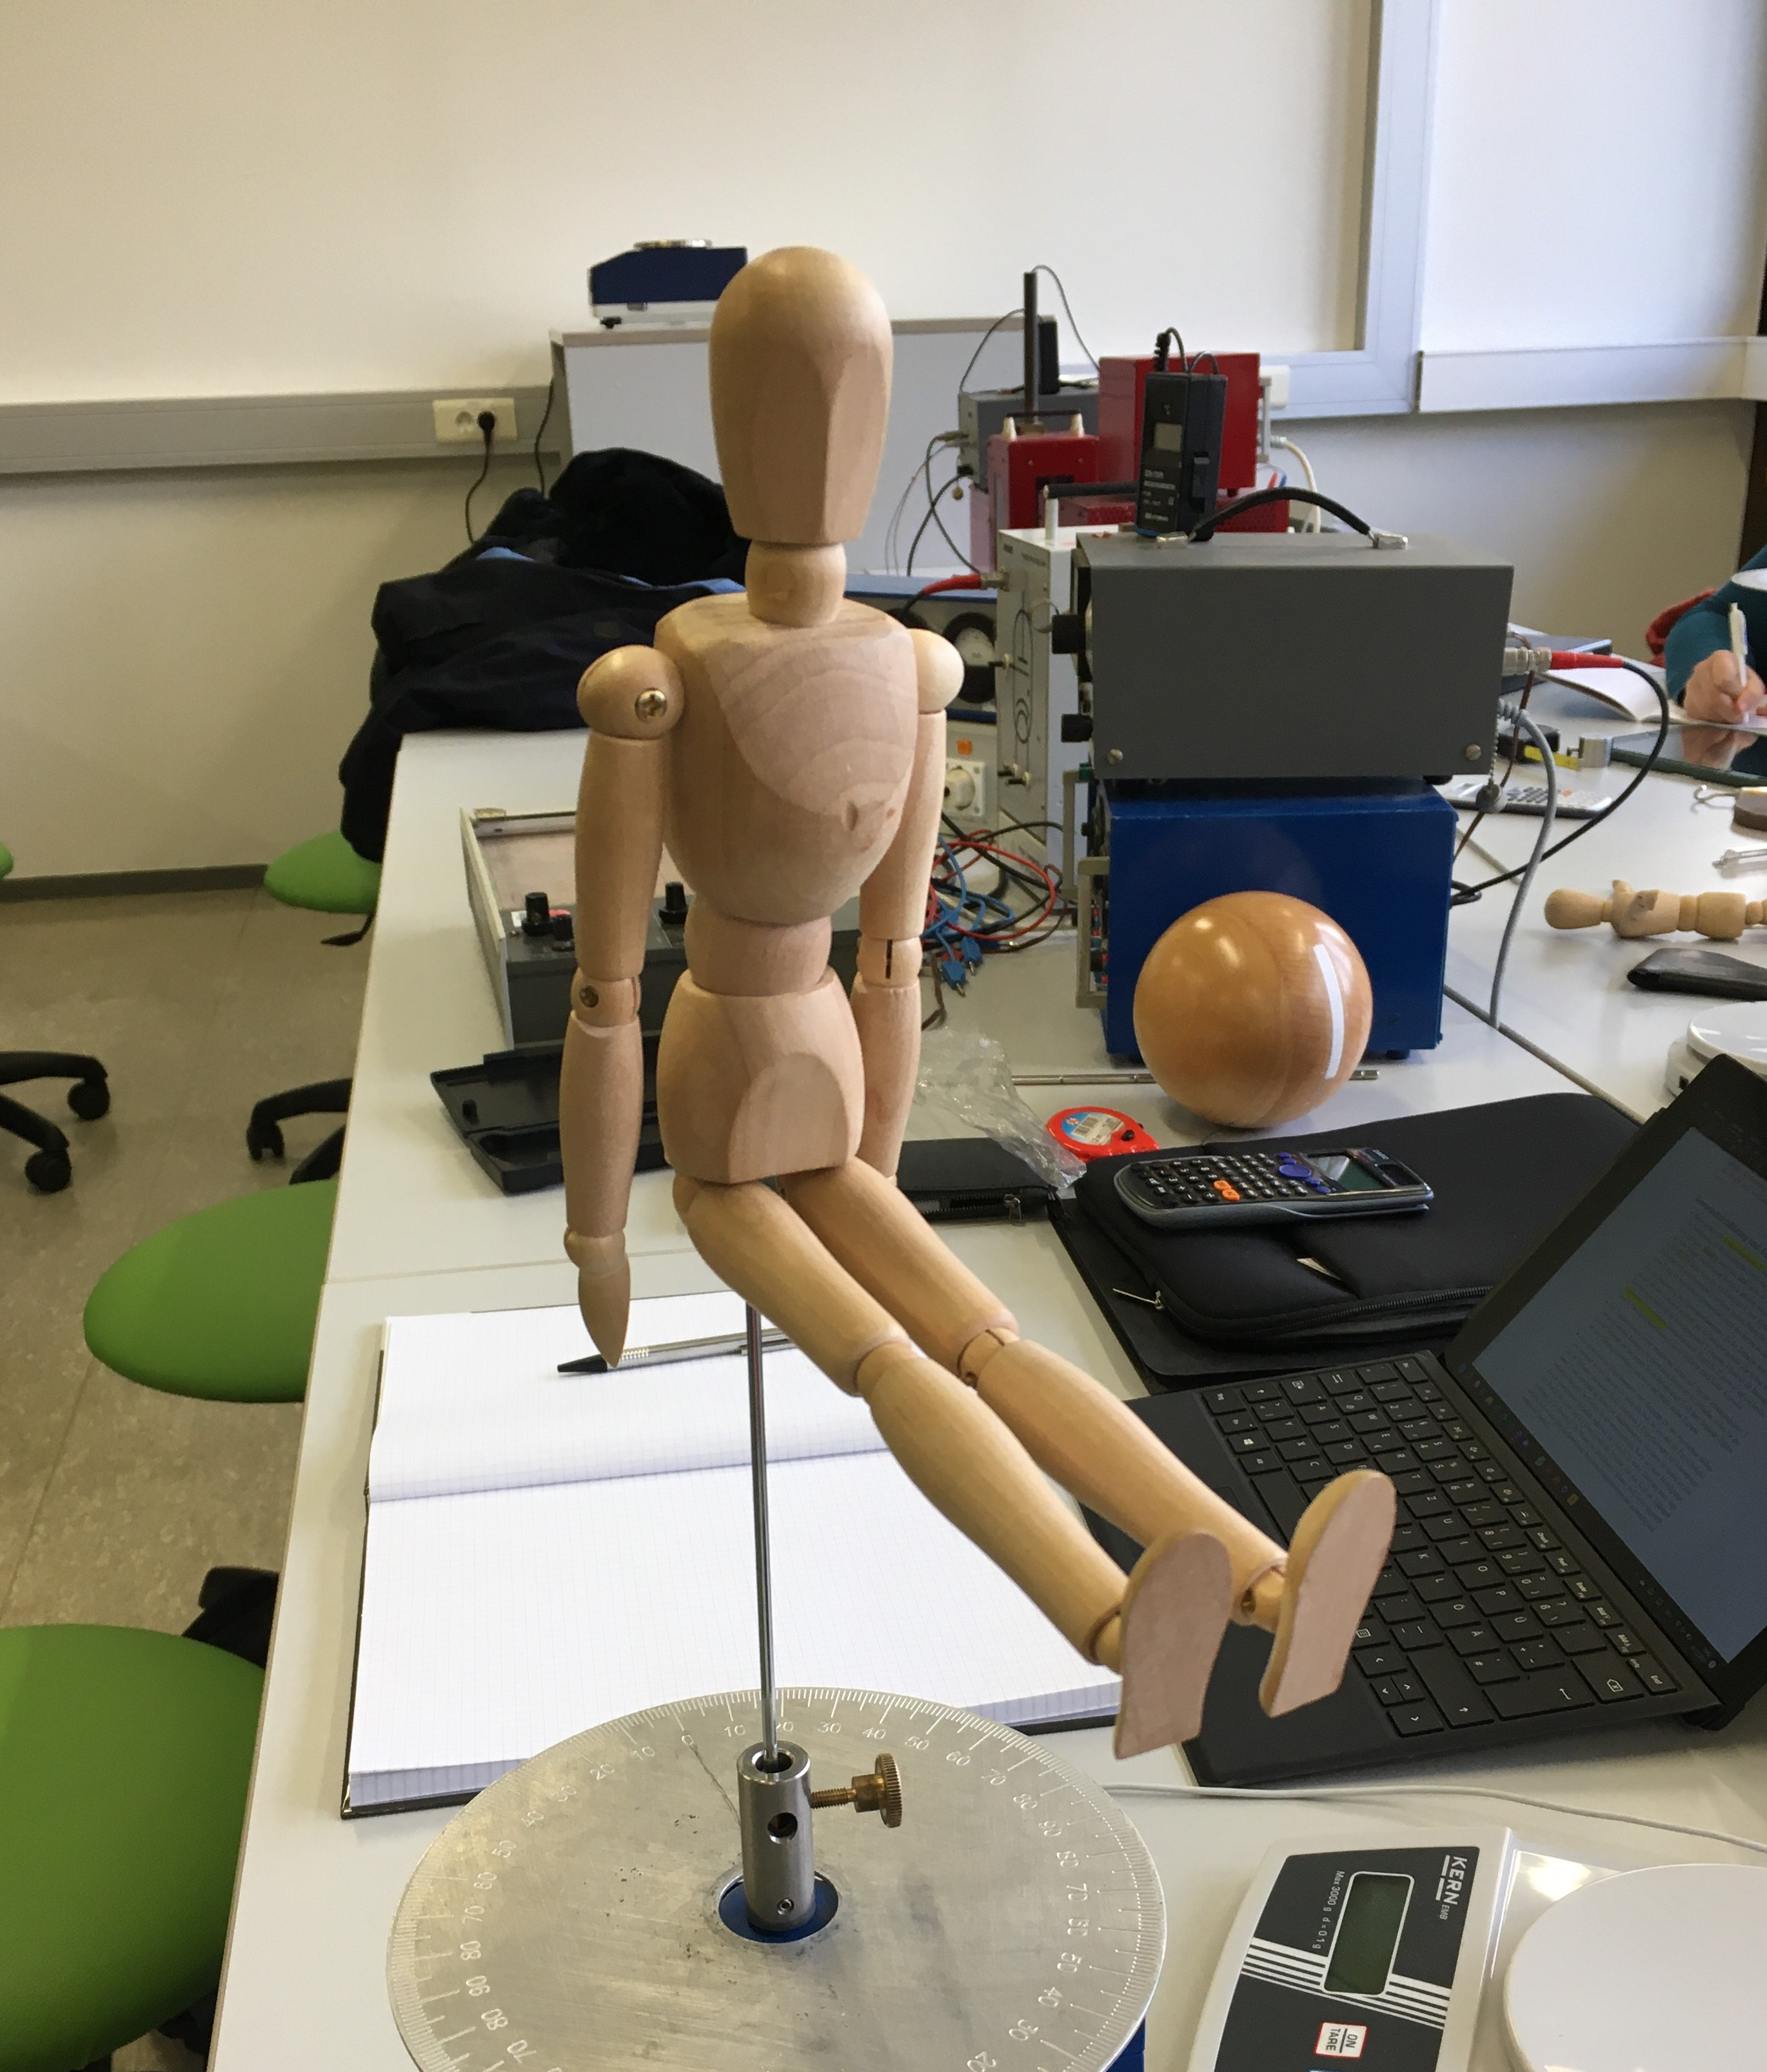
\includegraphics[width=0.3\columnwidth]{pictures/puppe_rechter_winkel.jpg}
  \caption{Die Puppe mit nach vorne gestrecken Beinen (90° Pose).}
  \label{fig:pose1}
\end{figure}

\begin{table}[H]
  \centering
  \caption{Messwerte der Periodendauer der ersten Pose.}
  \label{tab:PeriodendauerPose1}
  \begin{tabular}{rrr}
    \toprule
     & $T / \unit\second$ &  $T / \unit\second$  \\
    \midrule
    $\varphi$ : & 90° & 120° \\
    \midrule
          & 0,90 &        0,86 \\
          & 0,87 &        0,90 \\
          & 0,86 &        0,85 \\
          & 0,85 &        0,90 \\
          & 0,88 &        0,80 \\
    \midrule
    $T_{\text{mittel}}$ : & 0,872 & 0,862 \\
    \bottomrule
    \end{tabular}
\end{table}

Daraus lässt sich die gemittelte Schwingungsdauer
\begin{equation*}
  T_E = (0,867 \pm 0,02934) \, \unit\second
\end{equation*}
bestimmen.
Nun lässt sich das Trägheitsmoment berechnen.
Aus Gleichung (\ref{eq:Tumgestellt1}) und (\ref{fehler:gauß}) ergibt sich für das Trägheitsmoment

\begin{equation*}
  I_E =( 0,39985 \pm 0,07382) \cdot 10^{-3}  % FEHLER FEHLT
  \, \unit{\kilo\gram\meter\squared} \text{ .}
\end{equation*}

Nun wird das theoretische Trägheitsmoment berechnet.
Dafür wird zunächst das Trägheitsmoment der einzelnen Zylinder berechnet.
Dies leisten die Gleichungen
\begin{align*} \label{I_Puppe}
  I_{\text{Oberschenkel}} &= \frac{m_{\text{OS}} \cdot r_{\text{OS}}^2 + 2 \cdot m_{OS} \cdot r_{OS}^2} {2}  \text{ ,}\\
  I_{\text{Unterschenkel}} &= \frac{m_{\text{US}} \cdot r_{\text{US}}^2 + 2 \cdot m_{US} \cdot r_{US}^2} {2}  \text{ ,}\\
  I_{\text{Oberarm}} &= \frac{m_{\text{OA}} \cdot h_{\text{OA}^2} + 3 \cdot m_{\text{OA}} \cdot r_{\text{OK}}^2} {3}  \text{ und}\\
  I_{\text{Unterarm}} &= \frac{m_{\text{UA}} \cdot h_{\text{UA}^2} + 3 \cdot m_{\text{UA}} \cdot \left( r_{\text{OK}} + h_{\text{OA}}\right)^2} {3} \text{ .} \\
\end{align*}

Insgesamt ergibt sich damit
\begin{equation*}
  I_{\text{theo}} = (0,477969 \pm 0,00495) \cdot 10^{-3} \, \unit{\kilo\gram\meter\squared} \text{ .}
\end{equation*}

\subsubsection{Trägheitsmoment der Puppe: Pose 2}

Nun wird das Trägheitsmoment der Figur in der \enquote{T-Pose} untersucht.
Diese ist in Abbildung (\ref{fig:pose2}) dargestellt.
Zunächst wird die theoretische Erwartung berechnet.
Aus dem Satz von Steiner (\ref{eq:SatzvSteiner}) folgen die Gleichungen
\begin{align*}
I_{\text{Oberschenkel}} &= \frac{m_{\text{OS}} \cdot h_{\text{OS}}^2} {3} \text{ ,}\\
I_{\text{Unterschenkel}} &= \frac{m_{\text{US}} \cdot h_{\text{US}}^2 + 3 \cdot m_{US} \cdot h_{OS}^2} {3} \text{ ,}\\
I_{\text{Oberarm}} &= \frac{m_{\text{OS}} \cdot r_{\text{OS}^2} + 2 \cdot m_{\text{OA}} \cdot (r_{\text{OA}} + r_{\text{OK}})^2} {2} \text{ und}\\
I_{\text{Unterarm}} &= \frac{m_{\text{UA}} \cdot r_{\text{UA}^2} + 2 \cdot m_{\text{UA}} \cdot (r_{\text{UA}} + r_{\text{OK}})^2} {2} \text{ .}\\
\end{align*}

Damit lässt sich das Trägheitsmoment
\begin{equation*}
  I_{\text{theo}} = (0,13192 \pm 0,00672) \cdot 10^{-3} \, \unit{\kilo\gram\meter\squared}
\end{equation*}
berechnen.

\begin{figure}[H]
  \centering
  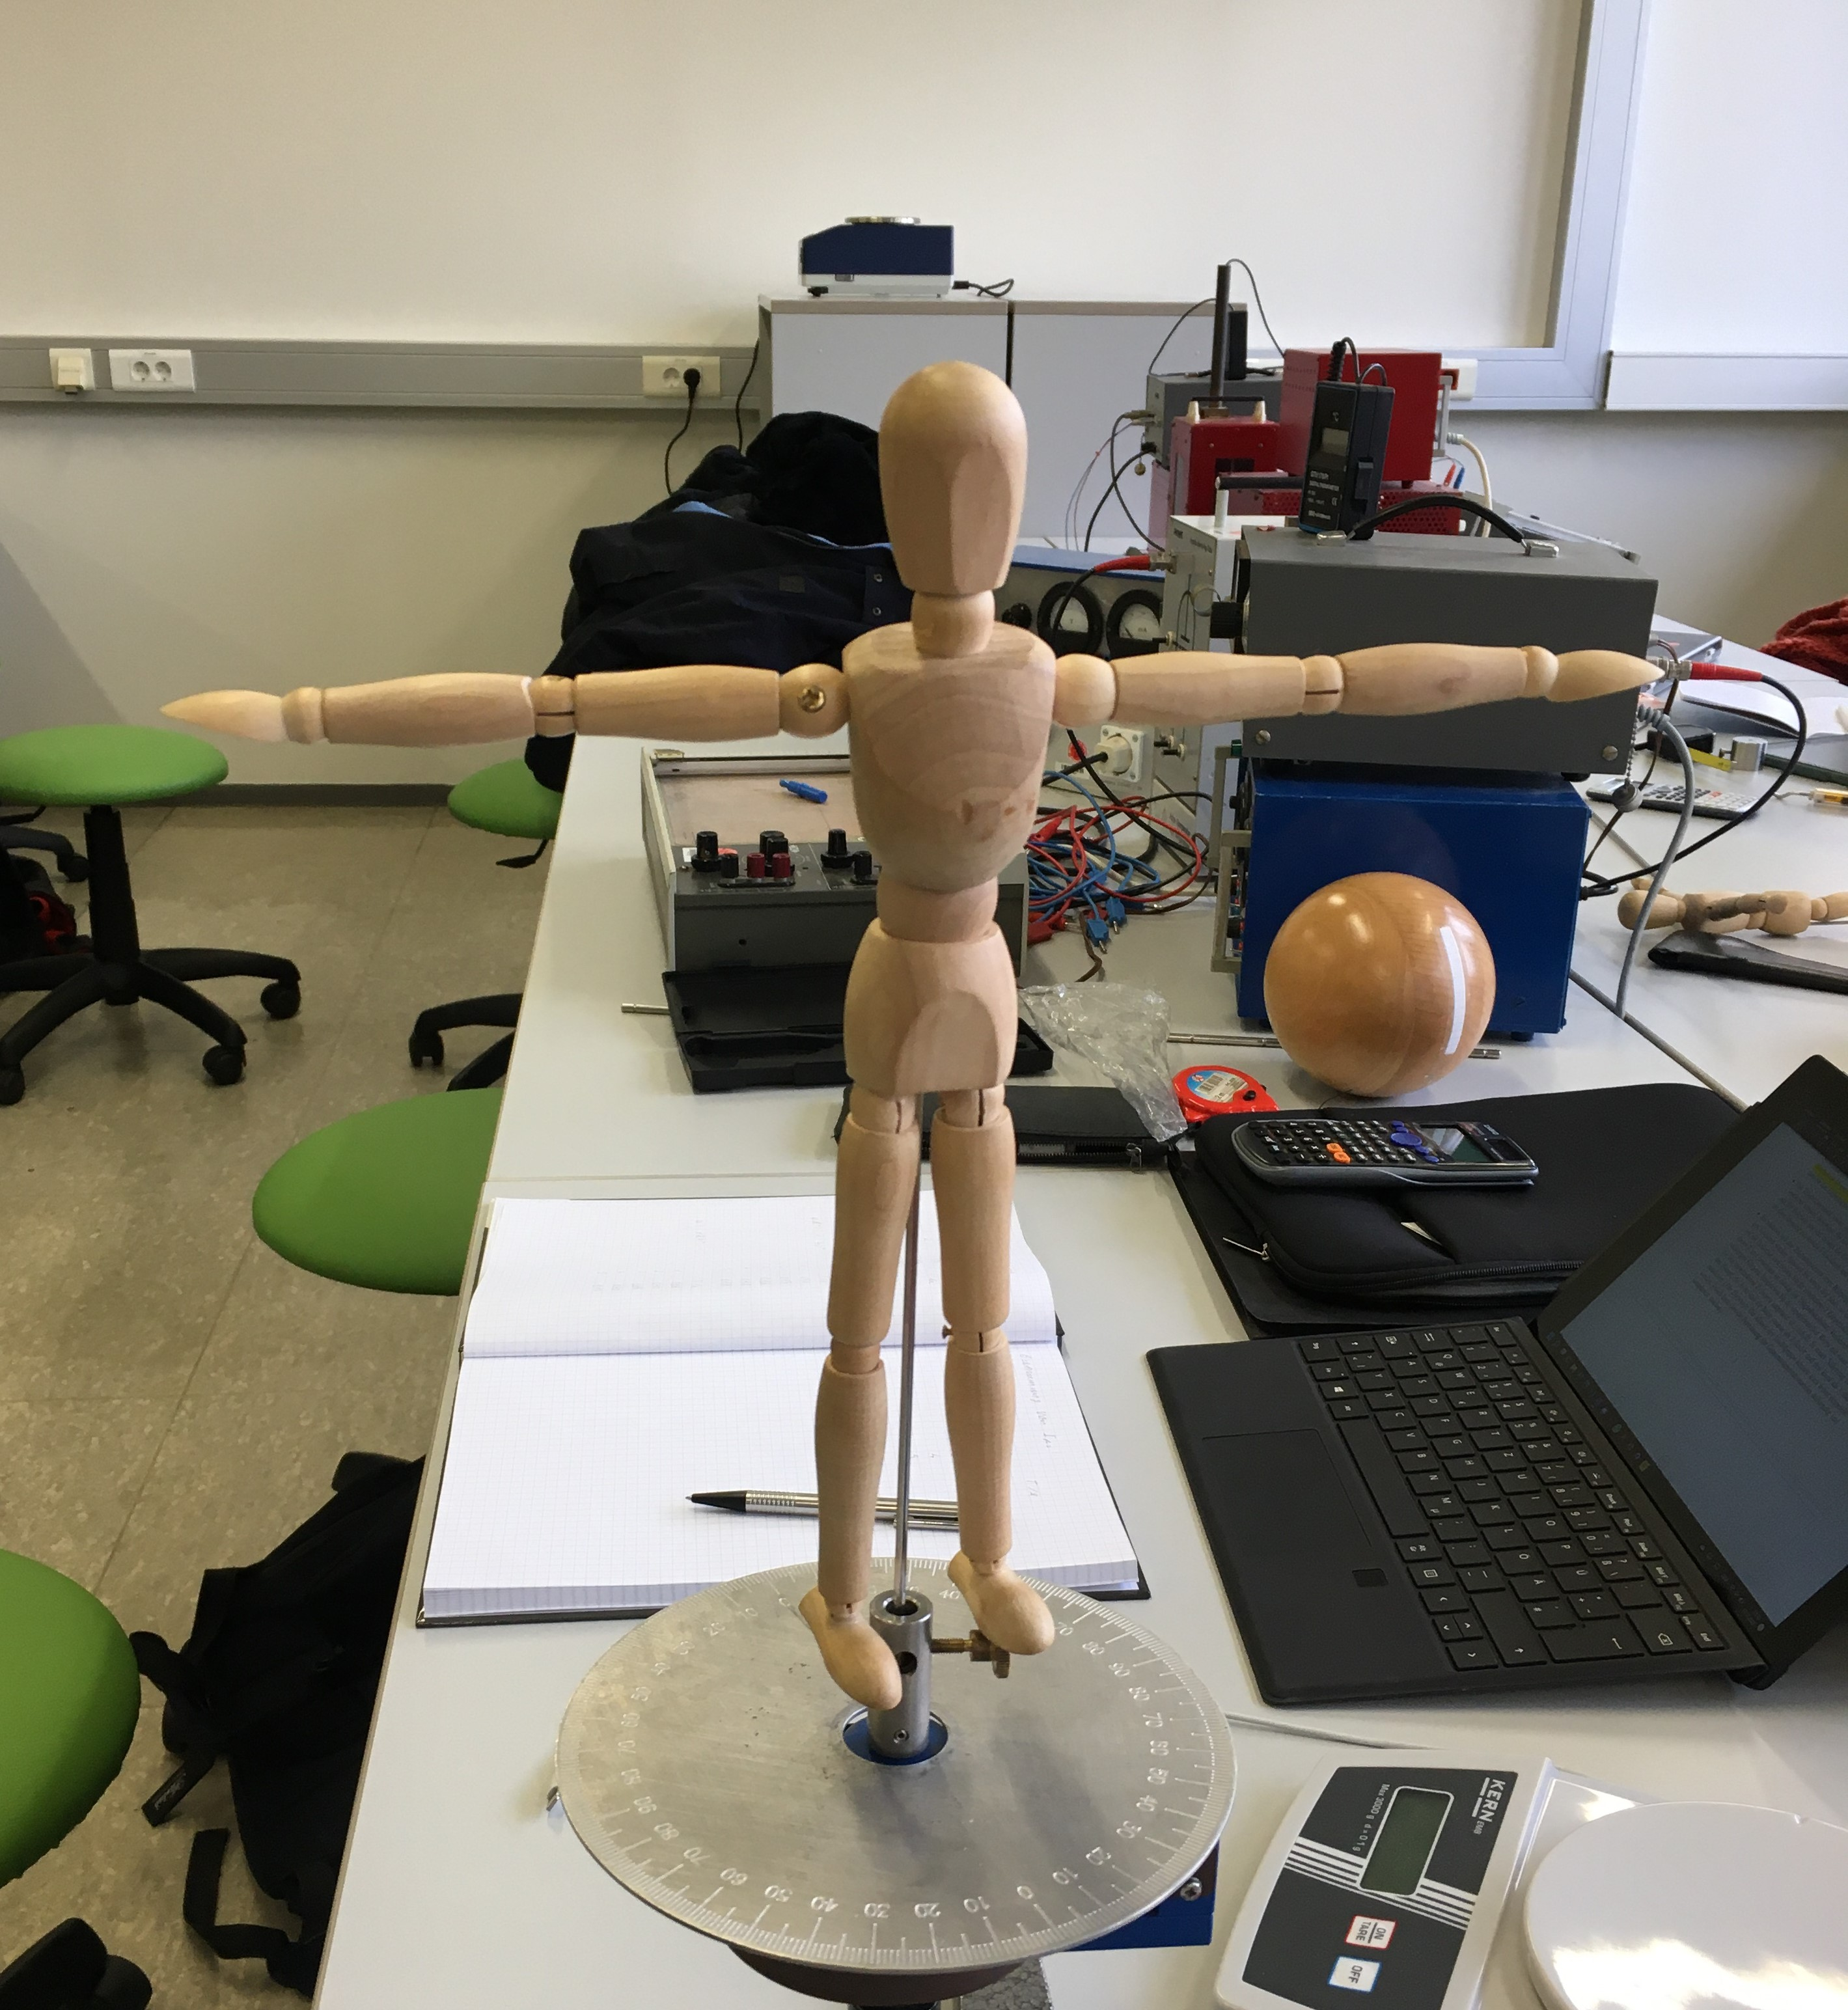
\includegraphics[width=0.3\columnwidth]{pictures/puppe_tpose.jpg}
  \caption{Die Puppe mit ausgestreckten Armen (\enquote{T-Pose})}
  \label{fig:pose2}
\end{figure}

\begin{table}
  \centering
  \caption{Messwerte der Periodendauer der zweiten Pose.}
  \label{tab:PeriodendauerPose2}
  \begin{tabular}{rrr}
    \toprule
    & $T / \unit\second$ &  $T / \unit\second$  \\
    \midrule
    $\varphi$ : & 90° & 120° \\
    \midrule
          & 0,64 &        0,70 \\
          & 0,70 &        0,67 \\
          & 0,66 &        0,68 \\
          & 0,67 &        0,70 \\
          & 0,65 &        0,71 \\
    \midrule
    $T_{\text{mittel}}$ : & 0,664 & 0,692 \\
    \bottomrule
    \end{tabular}
\end{table}

Nun lässt sich die Schwingungsdauer angeben zu
\begin{equation*}
  T_E = (0,678 \pm 0.02271) \, \unit\second \text{ .}
\end{equation*}

Daraus wiederum analog wie bei Pose 1 das Trägheitsmoment aus Gleichung (\ref{eq:Tumgestellt1}) und (\ref{fehler:gauß}) mit dem Wert

\begin{equation*}
  I_E = (0,24452 \pm 0,00524)  \cdot 10^{-3} % FEHLER FEHLT
  \, \unit{\kilo\gram\meter\squared} \text{ .}
\end{equation*}